
\subsection{Zillow}

\begin{frame}[label = zillow]
	\frametitle{Zillow Data}
	
	\begin{itemize}
		\item Leader online real estate and rental platform in the U.S. {\small (more 
		than 110 million homes and 170 million unique monthly users in 2019).}
		
		\vspace{2mm} \item
		Provides \textit{median} rents data at ZIP code, county, and state levels 
		at a monthly frequency for several housing categories.
		
		\pause
		\vspace{2mm} \item
		Use category single-family, condominium, and cooperative houses (SFCC):
		\begin{itemize}
			\item Most common housing type in the U.S.
			\item Most populated series in Zillow.
			%%\item Captures trends in metropolitan housing markets. 
			%%\hyperlink{zillow_safmr}{\beamerbutton{Comparison SAFMR}}
		\end{itemize}
		
		\pause
		\vspace{2mm} \item
		Limitation: Zillow sample is not random.
	\end{itemize}
\end{frame}

\begin{frame}[label = zipcodes_map]
	\frametitle{Comparison between Zillow Sample and Population Density}
	
	\vspace{-1mm}
	\begin{figure}
		\begin{subfigure}[t]{.49\textwidth}\centering
			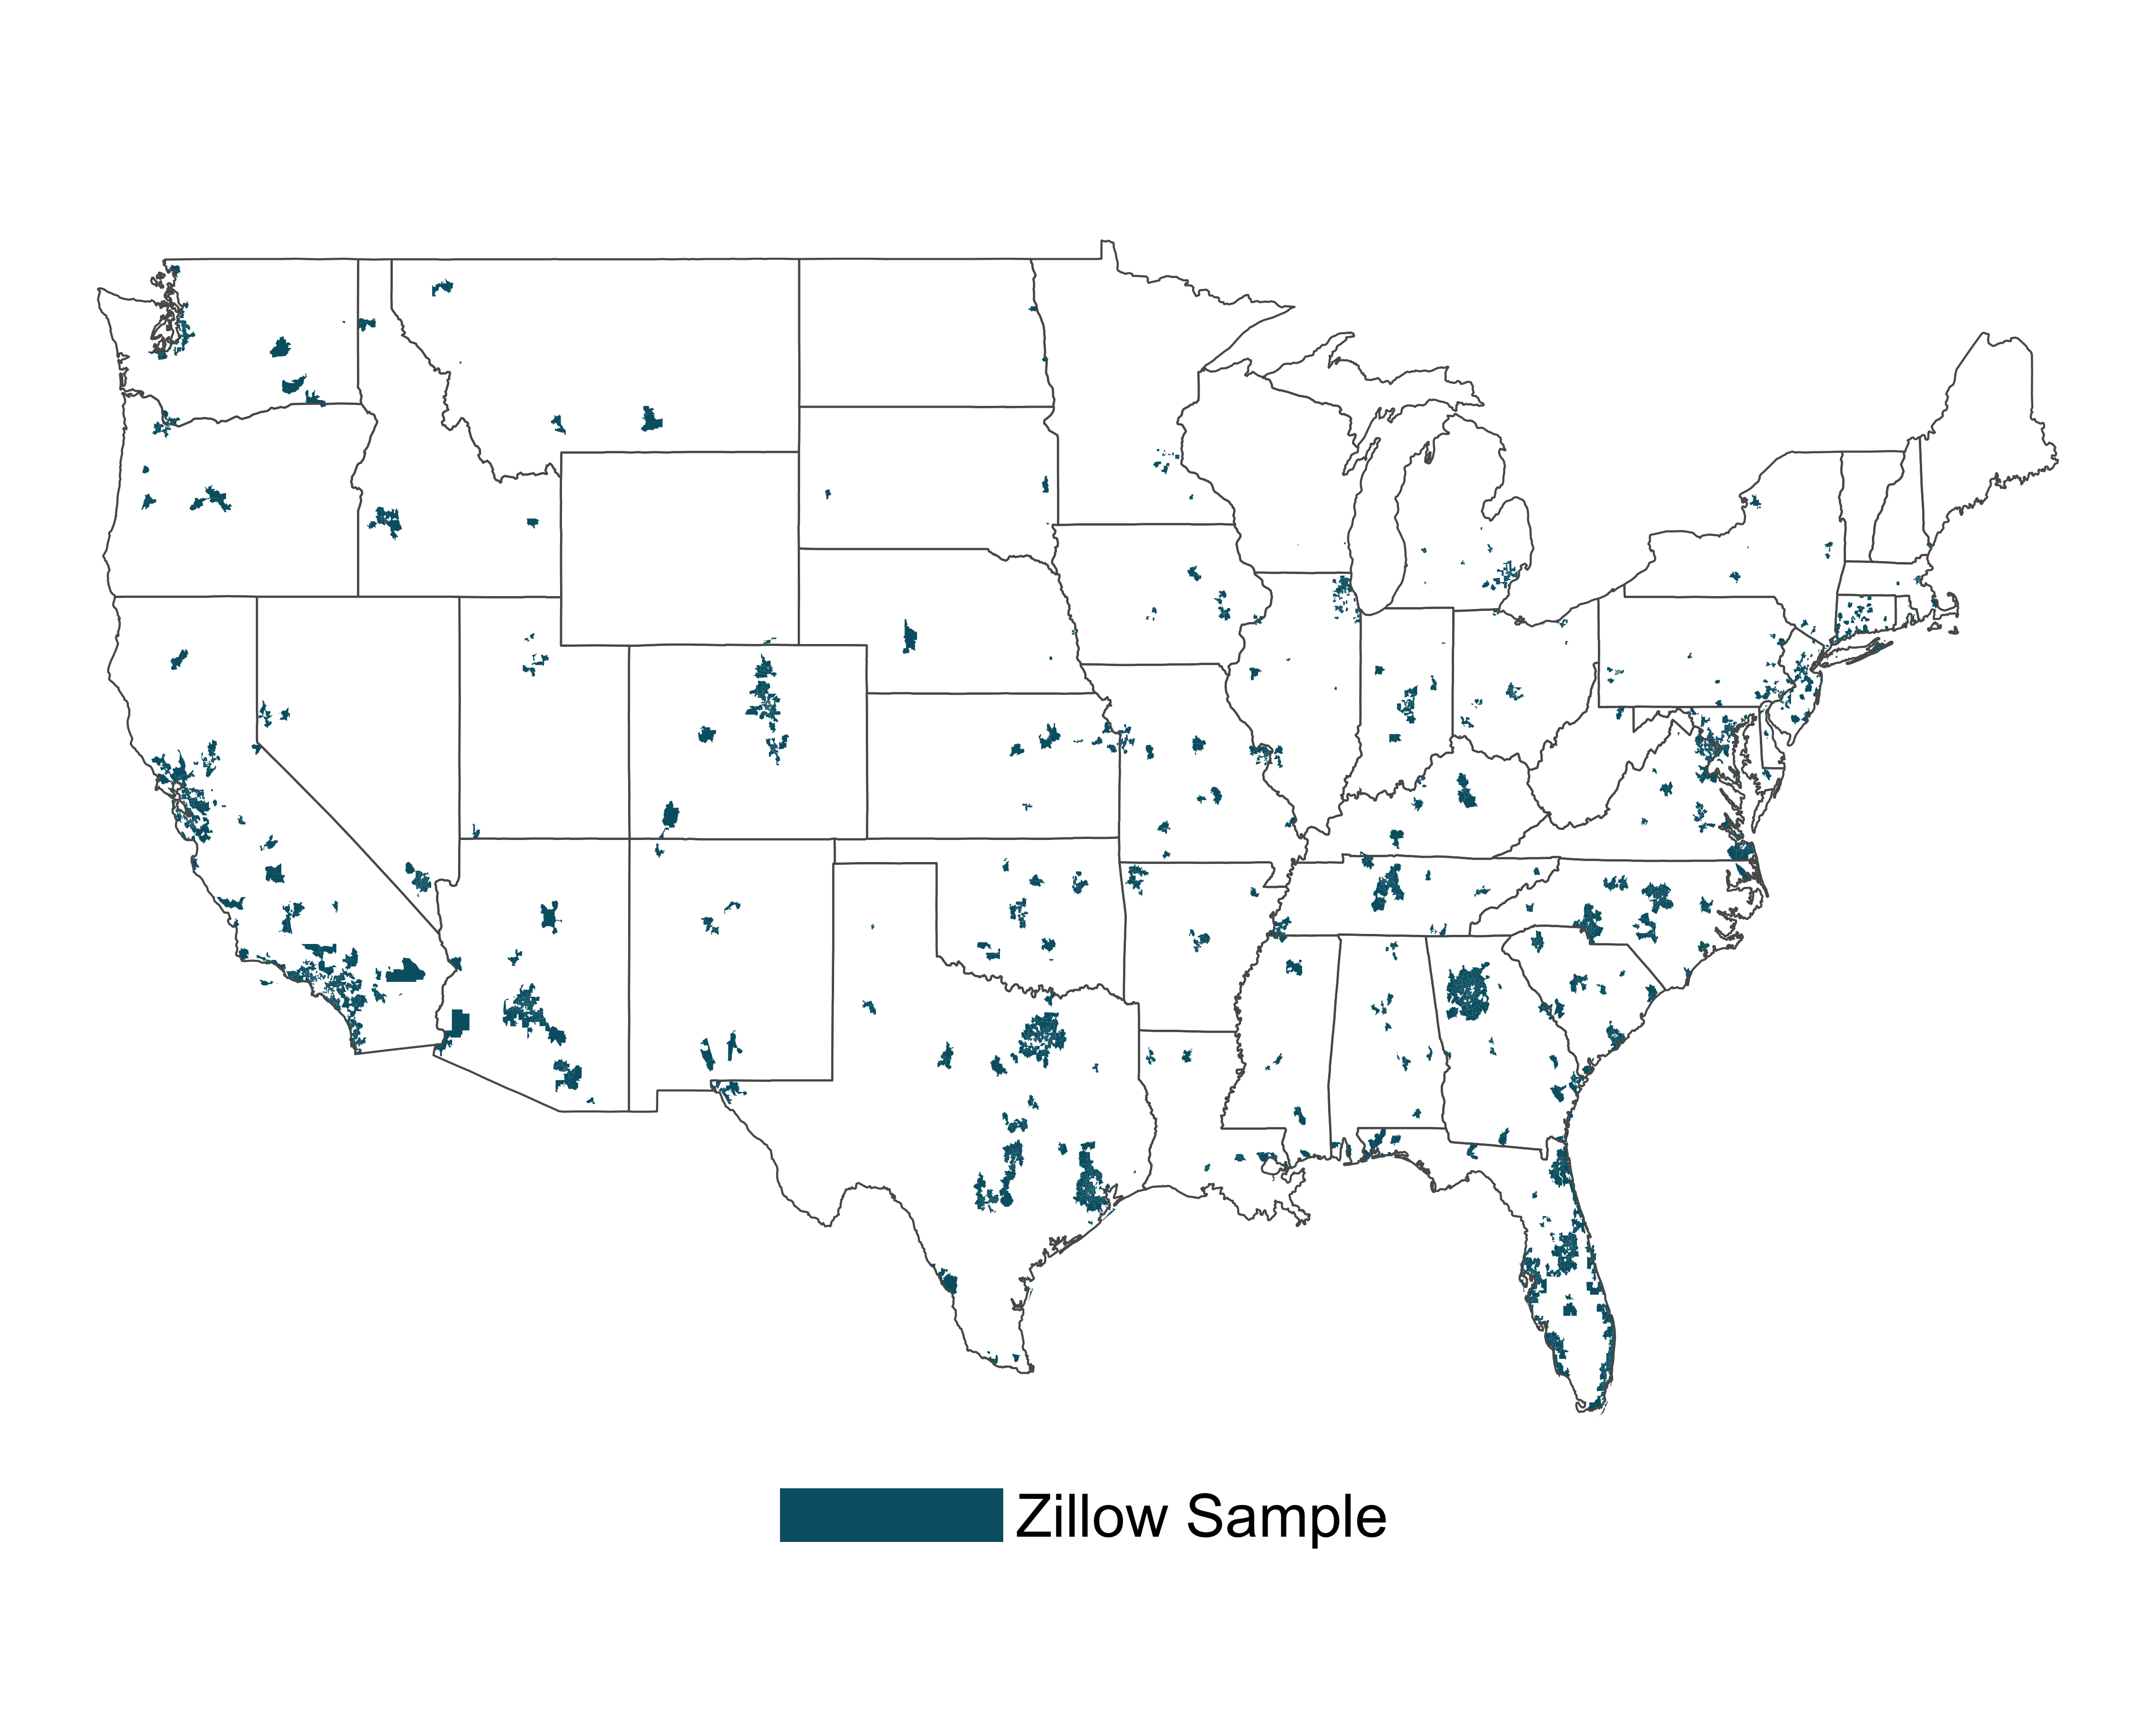
\includegraphics[width = .92\textwidth]
				{../../analysis/descriptive_maps/output/sample_map.png}
		\end{subfigure}
		\begin{subfigure}[t]{.49\textwidth}\centering
			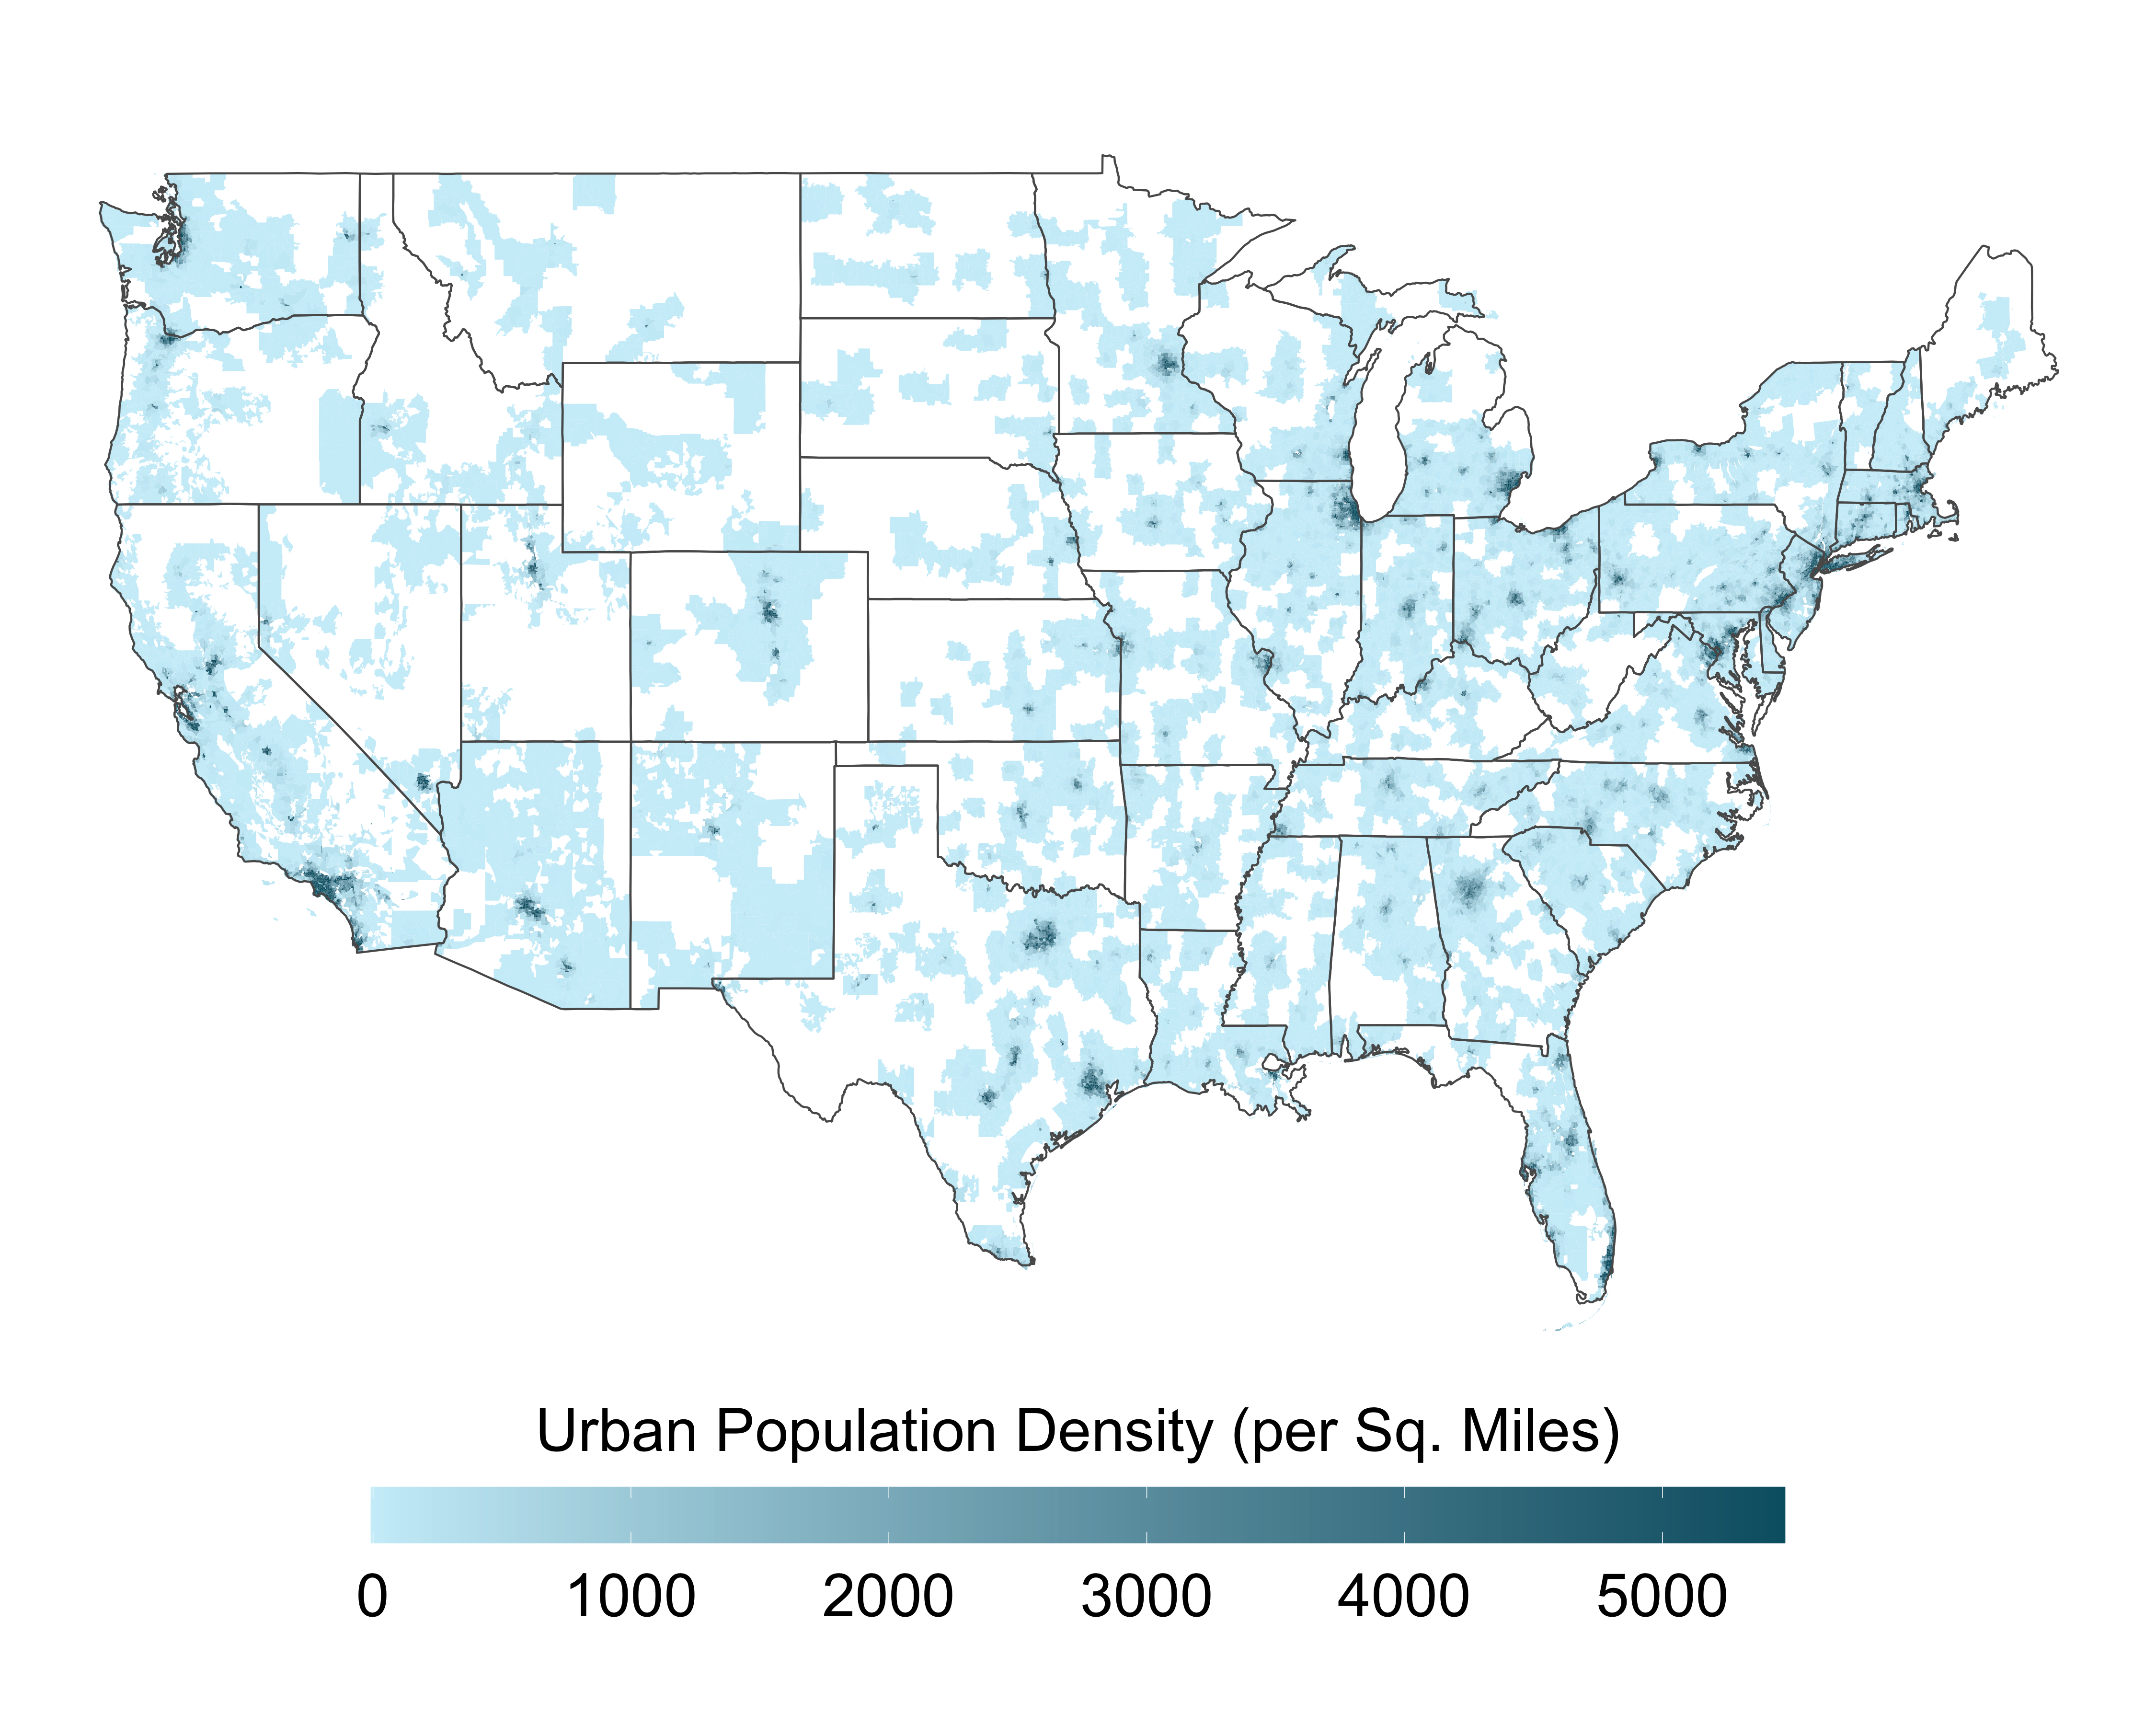
\includegraphics[width = .92\textwidth]
				{../../analysis/descriptive_maps/output/popurban_density_map.png}
		\end{subfigure}
		\begin{minipage}{.95\textwidth} \scriptsize	\vspace{1mm} 
			\textit{Notes}: Left panel shows ZIP codes available in Zillow data. Right 
			panel shows the urban population density for the top 100 metropolitan areas 
			in the U.S. from the 2008-2011 ACS (winsorized at the 99th percentile).
		\end{minipage}
	\end{figure}

	\hyperlink{tab_comparison}{\beamerbutton{Comparison Table}}

\end{frame}

% Should we add something about Zillow vs SAFMR? 

\subsection{Minimum Wages}

\begin{frame}[label=stat_MW]
	\frametitle{The Statutory MW}
	
	\begin{itemize}
		\item
		Collect MW data at state, county and city levels between Jan 2010 and Dec 2019.
		
		\vspace{2mm} \item
		Assign those data to ZIP codes.
		
		\vspace{2mm} \item
		Define statutory MW in ZIP code as maximum between state and local levels.
		
		\pause
		\vspace{2mm} \item
		ZIP codes available in Zillow contain 18,689 changes at the ZIP code-month level.
		\vspace{-3.5mm} 
		\begin{itemize} \small
			\item 151 state-level changes.
			\item 182 county- and city-level changes.
		\end{itemize}
		%% We use 4,224 events at the ZIP code-month level in our estimating panel
		
		\hyperlink{dist_mw_changes}{\beamerbutton{Distribution of MW changes}}
	\end{itemize}
	
\end{frame}

\begin{frame}
	\frametitle{Using LODES to construct the experienced log MW}
	
	Construct \textbf{origin-destination matrix} at ZIP code level from 2017 LODES.
	%% Original data comes at the block-group level
	Observe:
	\begin{itemize} \small
		\item Number of workers residing in a ZIP code and working in every other 
		ZIP code.
		\item Analogously, number of workers younger than 29 and earning less than 
		\$1,251.
		%% Exp MW constructed using any of these measures gives similar results
	\end{itemize}
	
	\pause
	\vspace{2.5mm}
	Define \textbf{experienced log MW} in ZIP code $i$ month $t$ as
	$$
	\underline{w}^{\text{exp}}_{it} = 
	\sum_{z \in \mathbb{Z}_i} \pi_{i z} \ln \underline{w}_{zt} \ ,
	$$
	%% IMPORTANT: We average the log of the MW! (Not log the average)
	\vspace{-2.5mm}
	where
	\vspace{1mm}
	\begin{itemize} \small
		\item $\mathbb{Z}_i$ are workplace locations of $i$'s residents, and
		\item $\pi_{i z} = \frac{L_{i z}}{L_i}$ is the share of $i$'s residents who work 
		in $z$.
	\end{itemize}
\end{frame}

\begin{frame}[label=san_diego_mw]
	\frametitle{The California MW Increase of January 2019 in San Diego} 
	
	%% San Diego MW Dec 2019: $11.5
	%% California MW Dec 2019: $11 (for large employers)
	%% Level MW Jan 2020 in both places: $12
	
	\begin{figure}
		\begin{subfigure}[b]{0.49\textwidth}
			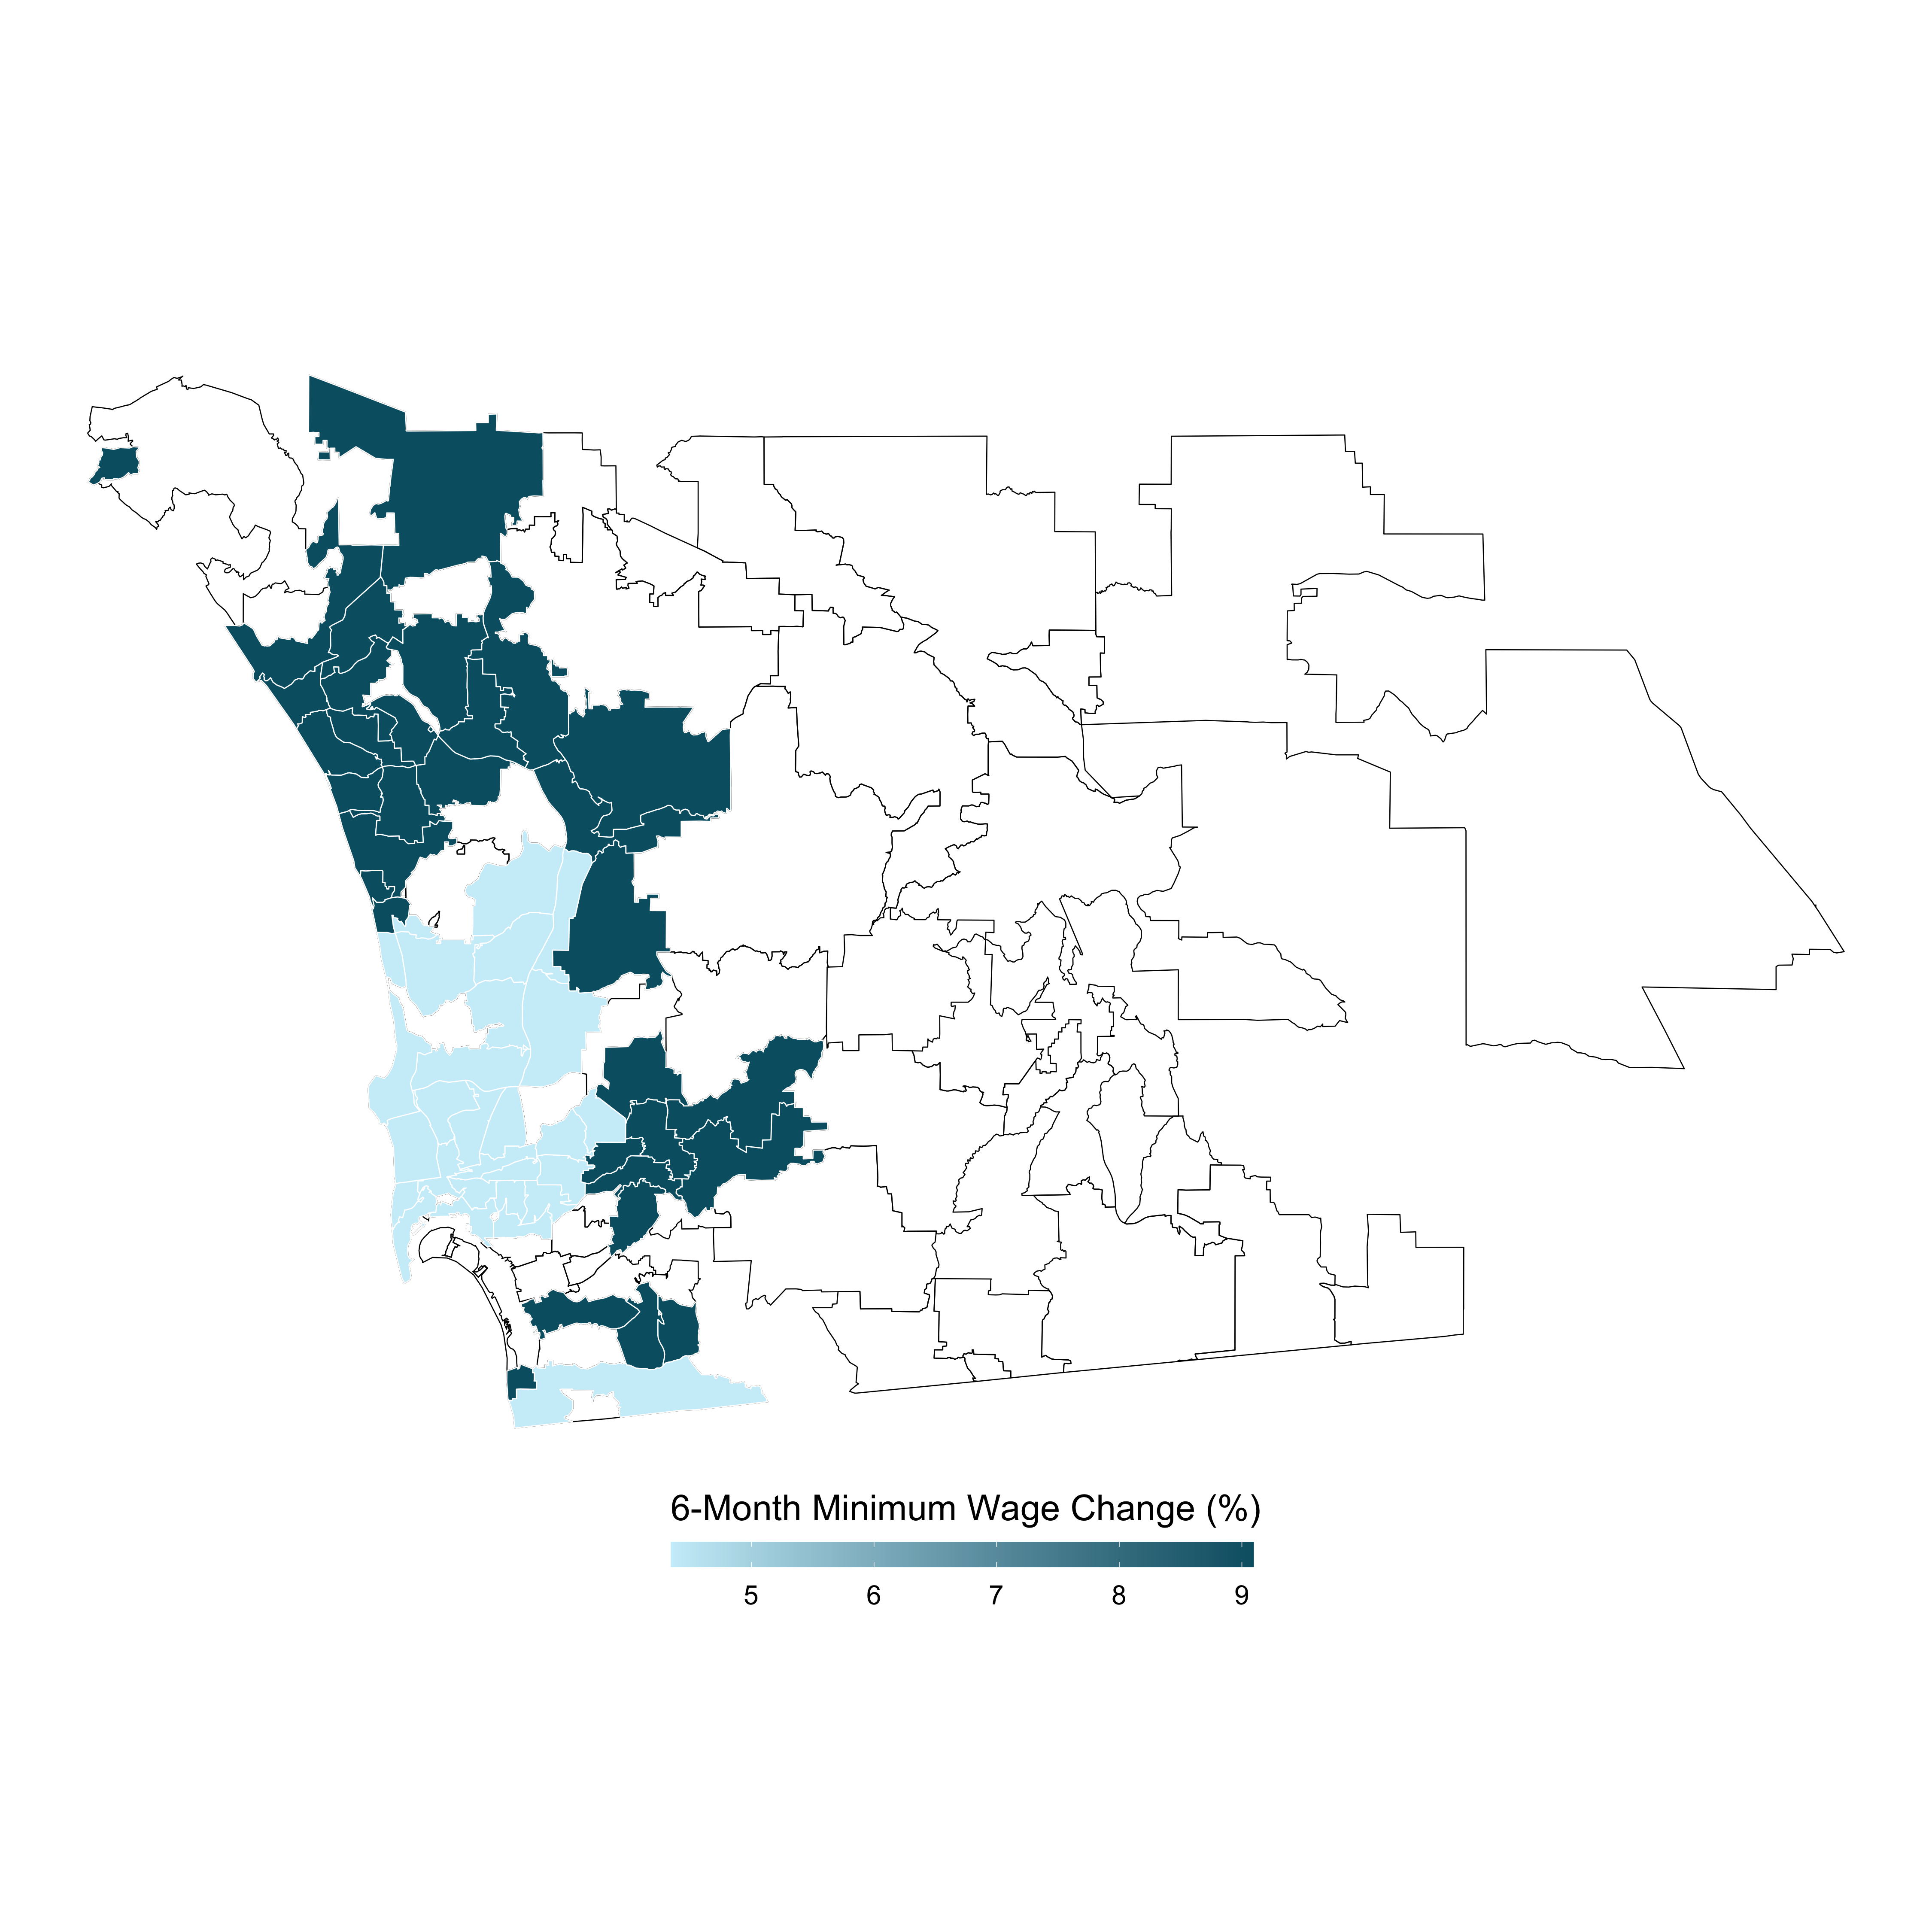
\includegraphics[width = .85\textwidth]
				{../../analysis/descriptive_maps/output/San_Diego_mw_msa.png}
		\end{subfigure}%
		\begin{subfigure}[b]{0.49\textwidth}
			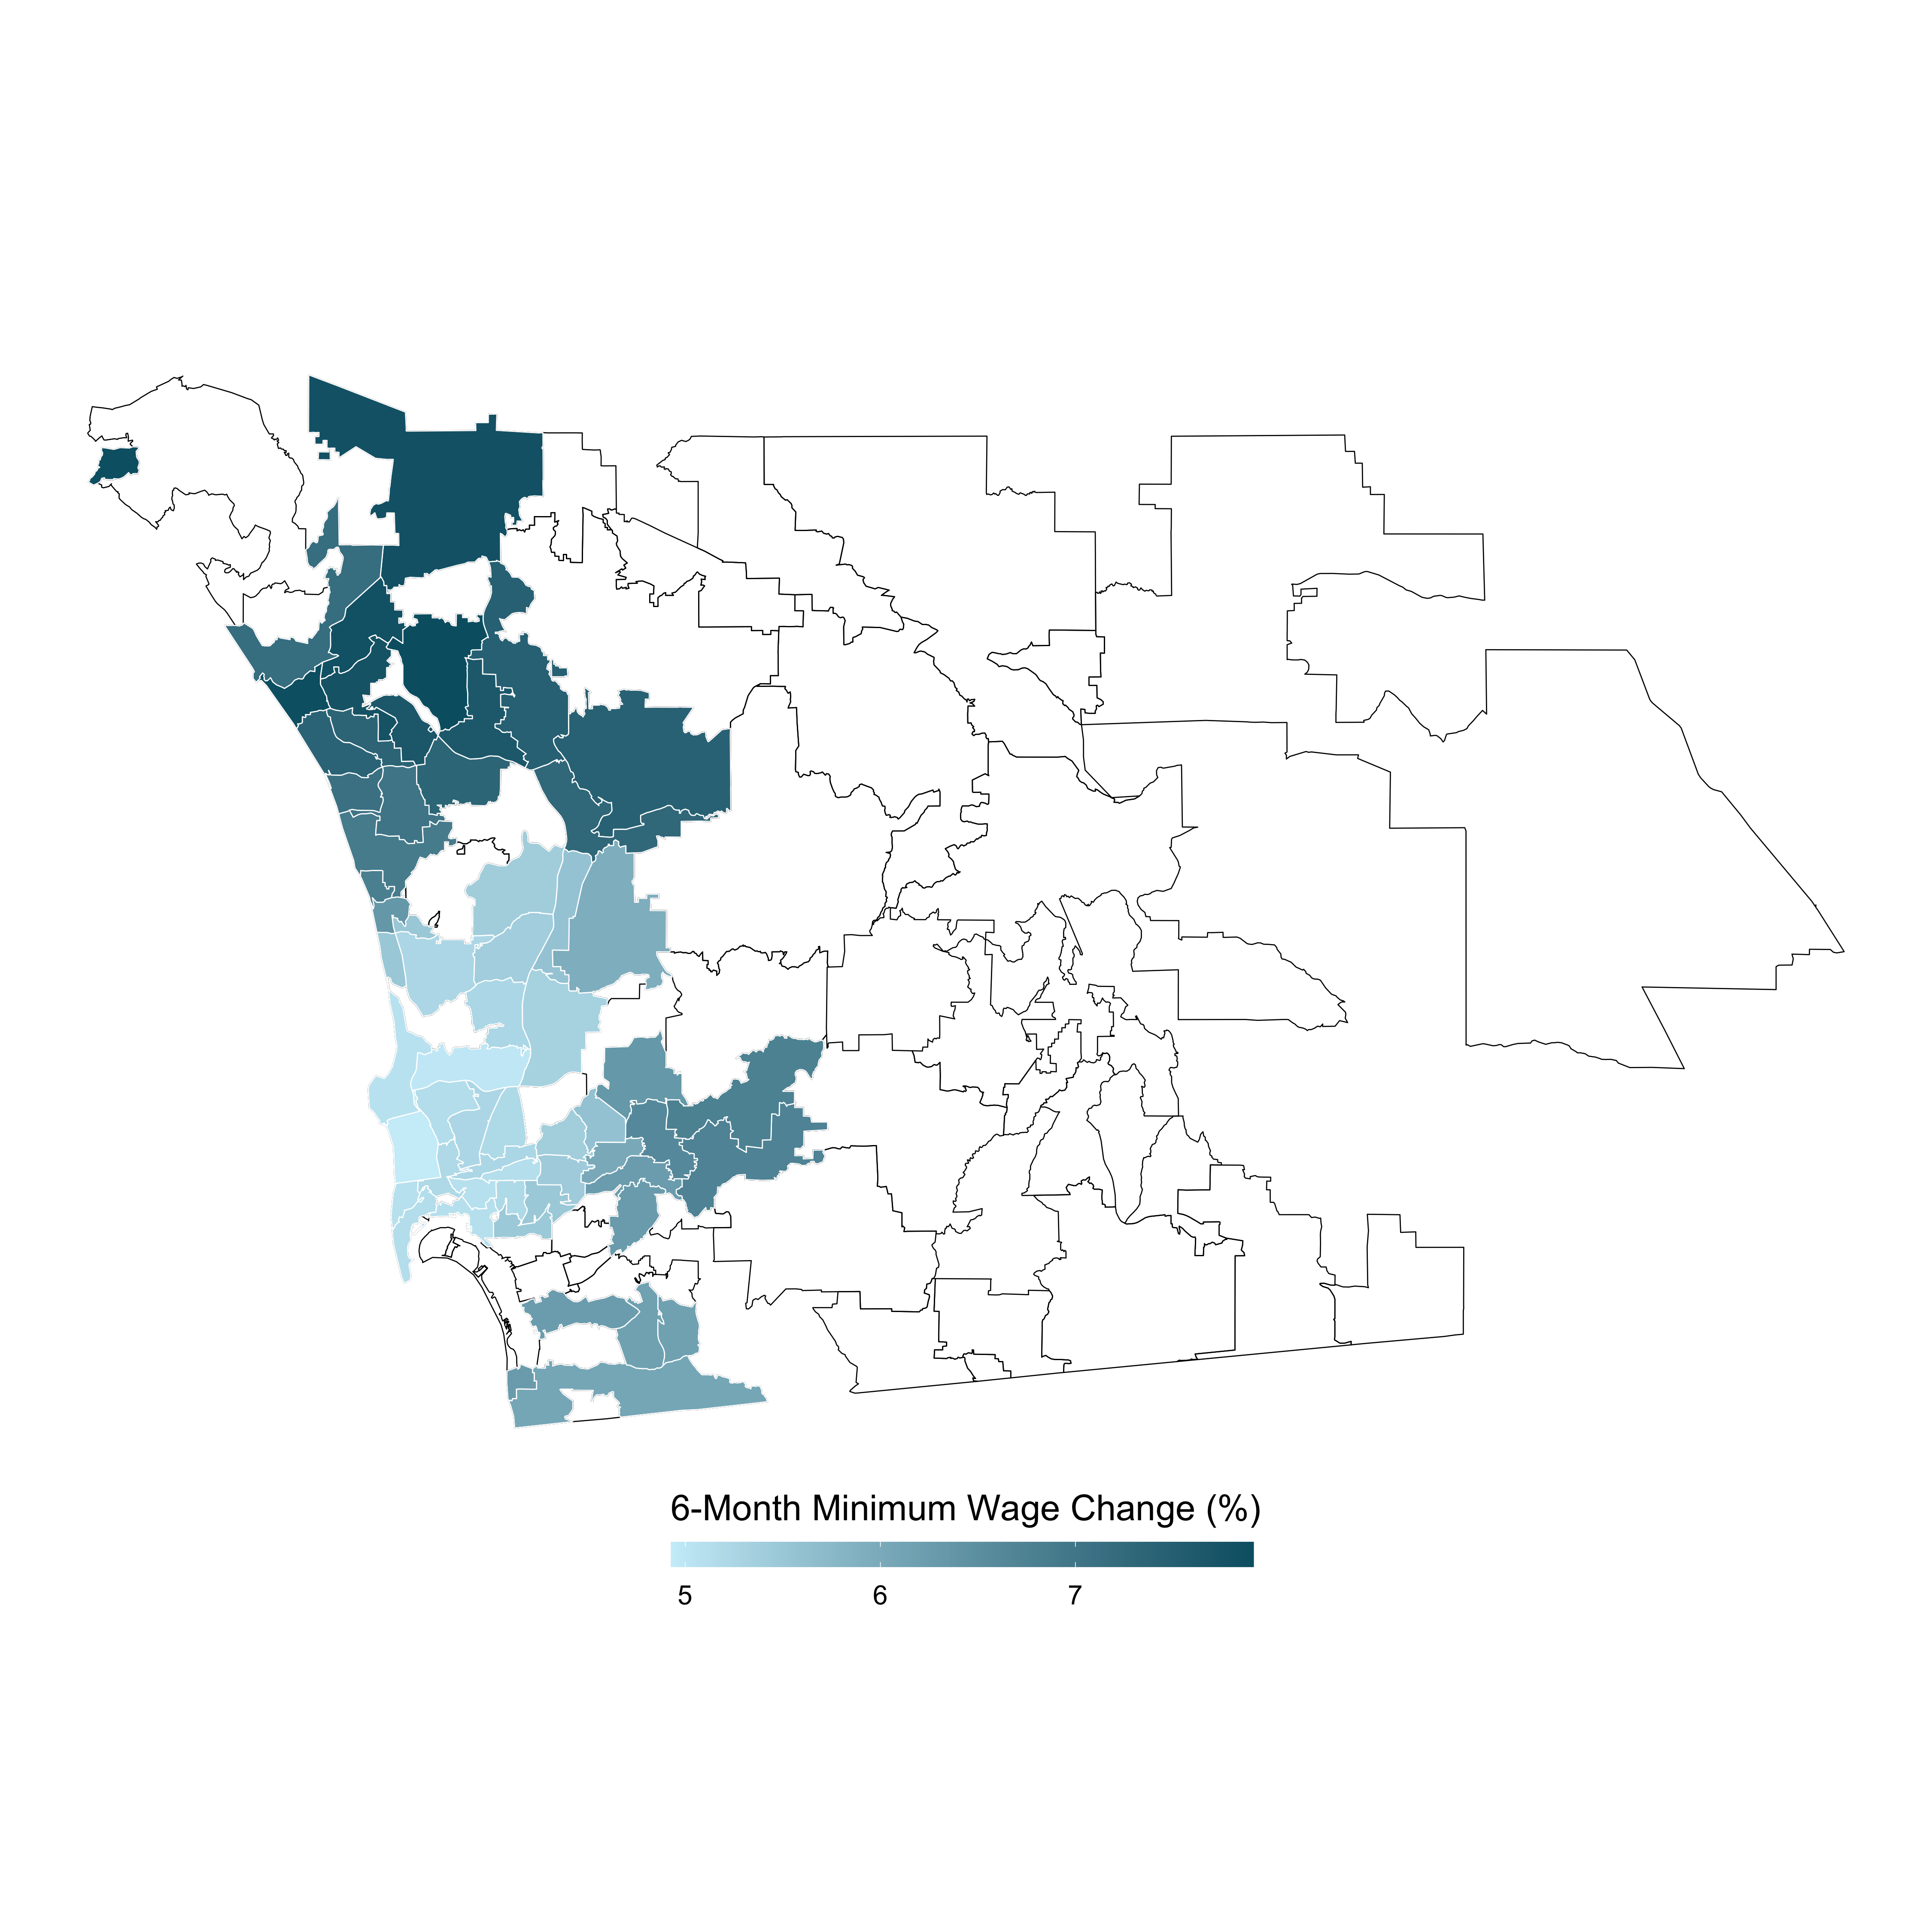
\includegraphics[width = .85\textwidth]
				{../../analysis/descriptive_maps/output/San_Diego_expmw_msa.png}
		\end{subfigure}
	\end{figure}
	
	\hyperlink{san_diego_rents}{\beamerbutton{Map rents}}
\end{frame}

\subsection{Sample Selection}

\begin{frame}[label=san_diego_mw]
	\frametitle{Other Data Sources and Sample Selection} 
	
	Other data sources:
	\begin{itemize}
		\item Economic controls from the Quarterly Census of Employment and Wages 
		{\small (QCEW)}.
	\end{itemize}
	
	\pause
	\vspace{3mm}
	ZIP codes enter Zillow data in different months.
	\begin{itemize} \small
		\item To account for composition changes in the sample, we use ZIP codes with 
		valid rents data as of July 2015 as baseline. (1,305 ZIP codes, 4,224 events.)
	\end{itemize}
	
	\vspace{2.5mm}
	We conduct several exercises changing the sample, and find consistent results.
%	\begin{itemize} \small
%		\item Use all ZIP codes available controlling for ``cohort $\times$ time-period'' 
%		fixed effects.
%		\item Use fully balanced panel starting from July 2015.
%		\item Weight regression to match key moments in the distribution of ZIP codes of 
%		top 100 CBSA.
%	\end{itemize}
	% Results are similar. Won't show everything for interest of time.
	
\end{frame}

\begin{frame}[label=san_diego_mw]
	\frametitle{Baseline Sample: Summary Statistics} 
	
	\begin{table}
		\scalebox{.87}{
% Table created by stargazer v.5.2.2 by Marek Hlavac, Harvard University. E-mail: hlavac at fas.harvard.edu
% Date and time: Mon, Nov 30, 2020 - 11:59:17 AM
\begin{tabular}{@{\extracolsep{5pt}}lccccc} 
\\[-1.8ex]\hline 
\hline \\[-1.8ex] 
Statistic & \multicolumn{1}{c}{N} & \multicolumn{1}{c}{Mean} & \multicolumn{1}{c}{St. Dev.} & \multicolumn{1}{c}{Min} & \multicolumn{1}{c}{Max} \\ 
\hline \\[-1.8ex] 
Statutory MW & 156,600 & 8.08 & 1.21 & 7 & 16 \\ 
Experienced MW & 156,600 & 8.06 & 1.20 & 6.29 & 14.98 \\ 
Median rent psqft. SFCC & 113,375 & 1.27 & 0.83 & 0.47 & 7.25 \\ 
Median rent SFCC & 125,644 & 1,651.10 & 702.99 & 595.00 & 6,595.00 \\ 
Avg. wage Fin. activities & 152,334 & 1,561.78 & 965.27 & 0.00 & 9,557.00 \\ 
Employment Fin. activities & 152,334 & 59,554.22 & 75,796.09 & 0.00 & 397,839.00 \\ 
Estab. count Fin. activities & 152,334 & 5,103.83 & 5,200.06 & 31.00 & 30,405.00 \\ 
\hline \\[-1.8ex] 
\end{tabular} 
}
		\vspace{4mm}
		\begin{minipage}{0.95\textwidth} \scriptsize
			Notes: The table shows summary statistics of some variables in our baseline 
			estimating sample, which includes 1,305 ZIP codes and runs from January 2010 
			to December 2019.
		\end{minipage}
	\end{table}
\end{frame}
